\documentclass{beamer}
\usepackage{amsmath,amsbsy,amsopn,amstext,amsfonts,amssymb}
\usepackage{isomath}
\usepackage{ulem}
%\linespread{1.6}  % double spaces lines
\usepackage{graphicx}
\usepackage{subfigure}
\usepackage{color}
\usepackage{optidef}  % define optimization problems
\usepackage{multicol}  % multiple columns
\usepackage{listings} % for python code
\usepackage{mathrsfs}

\usepackage{polynom}
\newcommand{\adj}{\mathrm{adj}}
\newcommand{\constrainedmin}[3]{
		\begin{mini*}|s|
		{#2}{#1}{}{}
		\addConstraint{#3}
		\end{mini*}
}

\newcommand{\rwbcomment}[1]{{\color{blue}RWB:#1}}
\newcommand{\defeq}{\stackrel{\triangle}{=}}
\newcommand{\abs}[1]{\left|#1\right|}
\newcommand{\norm}[1]{\left\|#1\right\|}
\newcommand{\iprod}[1]{\left<#1\right>}
\newcommand{\ellbf}{\boldsymbol{\ell}}
\newcommand{\nubf}{\boldsymbol{\nu}}
\newcommand{\mubf}{\boldsymbol{\mu}}
\newcommand{\abf}{\mathbf{a}}
\newcommand{\bbf}{\mathbf{b}}
\newcommand{\cbf}{\mathbf{c}}
\newcommand{\dbf}{\mathbf{d}}
\newcommand{\ebf}{\mathbf{e}}
\newcommand{\fbf}{\mathbf{f}}
\newcommand{\gbf}{\mathbf{g}}
\newcommand{\hbf}{\mathbf{h}}
\newcommand{\ibf}{\mathbf{i}}
\newcommand{\jbf}{\mathbf{j}}
\newcommand{\kbf}{\mathbf{k}}
\newcommand{\lbf}{\mathbf{l}}
\newcommand{\mbf}{\mathbf{m}}
\newcommand{\nbf}{\mathbf{n}}
\newcommand{\obf}{\mathbf{o}}
\newcommand{\pbf}{\mathbf{p}}
\newcommand{\qbf}{\mathbf{q}}
\newcommand{\rbf}{\mathbf{r}}
\newcommand{\sbf}{\mathbf{s}}
\newcommand{\tbf}{\mathbf{t}}
\newcommand{\ubf}{\mathbf{u}}
\newcommand{\vbf}{\mathbf{v}}
\newcommand{\wbf}{\mathbf{w}}
\newcommand{\xbf}{\mathbf{x}}
\newcommand{\ybf}{\mathbf{y}}
\newcommand{\zbf}{\mathbf{z}}
\newcommand{\Jbf}{\mathbf{J}}
\newcommand{\Acal}{\mathcal{A}}
\newcommand{\Bcal}{\mathcal{B}}
\newcommand{\Lcal}{\mathcal{L}}
\newcommand{\Ncal}{\mathcal{N}}
\newcommand{\Rcal}{\mathcal{R}}
\definecolor{darkolivegreen}{rgb}{0.33, 0.42, 0.18}

\makeatletter
\newenvironment<>{proofstart}[1][\proofname]{%
    \par
    \def\insertproofname{#1\@addpunct{.}}%
    \usebeamertemplate{proof begin}#2}
  {\usebeamertemplate{proof end}}
\newenvironment<>{proofcont}{%
  \setbeamertemplate{proof begin}{\begin{block}{}}
    \par
    \usebeamertemplate{proof begin}}
  {\usebeamertemplate{proof end}}
\newenvironment<>{proofend}{%
    \par
    \pushQED{\qed}
    \setbeamertemplate{proof begin}{\begin{block}{}}
    \usebeamertemplate{proof begin}}
  {\popQED\usebeamertemplate{proof end}}
\makeatother

\title{ECEn 671: Mathematics of Signals and Systems}
\author{Randal W. Beard}
\institute{Brigham Young University}
\date{\today}

\begin{document}

%-------------------------------
\begin{frame}
	\titlepage
\end{frame}



%%%%%%%%%%%%%%%%%%%%%%%%%%%%%%%%%%%%%%%%%%%%%%%%%%%%%%%%%%%%%%%%%
\section{Applications}
\frame{\sectionpage}

%----------------------------------
\begin{frame}\frametitle{Application:  Total least squares}
	If we are trying to fit a line to
	\[ 
		y_i = ax_i
	\]
	where $(y_i,x_i)$ are measured.  The least squares solution minimizes $e_i = y_i-ax_i$.
	Therefore $y_i - e_i = ax_i$.
	\begin{center}
		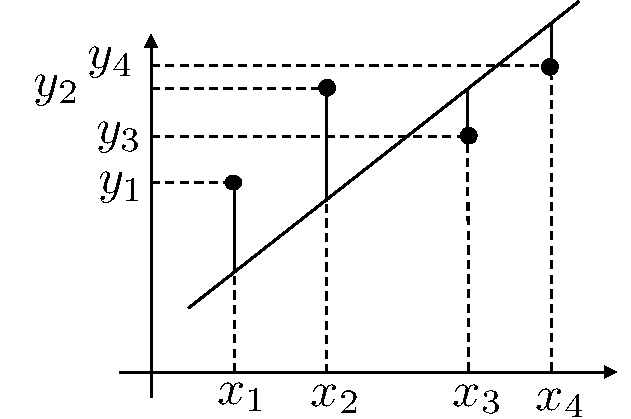
\includegraphics[width=0.5\textwidth]
			{figures/chap7_total_least_squares}
	\end{center}
	In other words: fix the $x_i$'s and play with $a$ to minimize the error.	
\end{frame}

%----------------------------------
\begin{frame}\frametitle{Application:  Total least squares}
	For the general problem $\min \norm{Ax - b}$ we assume $A$ is perfect and that the imperfection is completely in $b$
	\begin{center}
		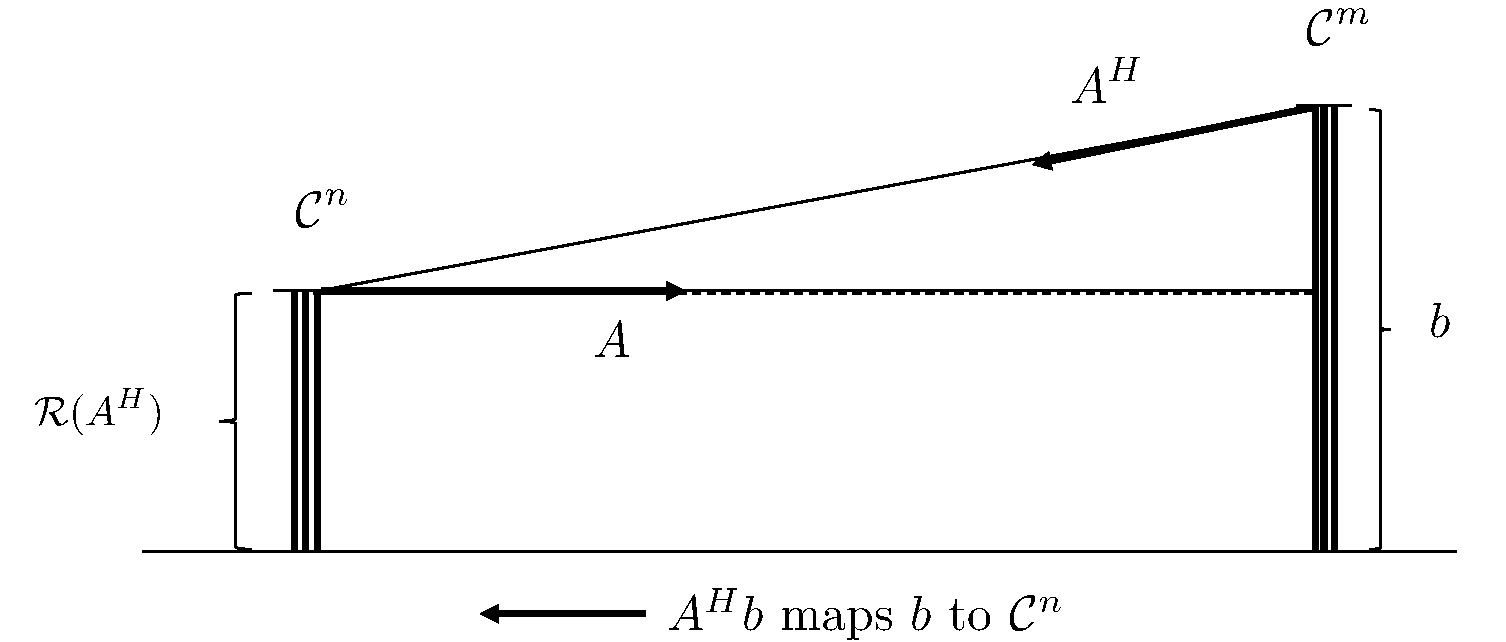
\includegraphics[width=0.5\textwidth]{figures/chap7_svd_2}
	\end{center}
	Recall $A^HAx = A^Hb$.  When we premultiply by $A^H$ we zero everything in $b$ that was in the null space of $A^H$ (i.e. we get rid of the bad parts of $b$).	
\end{frame}

%----------------------------------
\begin{frame}\frametitle{Application:  Total least squares}
	However $A$ often comes from noisy data as well (like when fitting a line to data) e.g. if $\ubf_i = ax_i+b$, then
	\[ 
		\begin{pmatrix}
	    	y_1\\
	    	\vdots\\
	    	\underbrace{y_n}_{\text{noisy}}
	  	\end{pmatrix} 
	  	= \begin{pmatrix}
	    	x_1 & 1\\
	    	\vdots & \vdots \\
	    	\underbrace{x_n}_{\text{noisy}} 
	    	& \underbrace{1}_{\text{perfect}}
	  	  \end{pmatrix}
	  	  \begin{pmatrix}
	    	a\\b
	  	  \end{pmatrix}
	\]	
\end{frame}

%----------------------------------
\begin{frame}\frametitle{Application:  Total least squares}
	Another interpretation of least squares is to find the \underline{smallest} perturbation of $b$, i.e., $\delta b$ such that
	\[ 
		Ax = b + \delta b 
	\] 
	where $b + \delta b \in \mathcal{R}(A)$.
	
	\vfill
	
	The total lest squares problem is to find the smallest perturbation of $b$ and $A$, denoted $\delta b$, $\delta A$ such that
	\[ 
		(A + \delta A)x = (b + \delta b) 
	\]
	supposing that $\begin{pmatrix} A & b \end{pmatrix}$ is full rank.
\end{frame}

%----------------------------------
\begin{frame}\frametitle{Application:  Total least squares}
	This can be written as
	\[ 
		\begin{pmatrix}
	    	A & b
	  	\end{pmatrix}
	  	\begin{pmatrix}
	    	x \\ -1
	  	\end{pmatrix}
	  + \begin{pmatrix}
	    	\delta A & \delta b
	  	\end{pmatrix}
	  	\begin{pmatrix}
	    	x \\-1
	  	\end{pmatrix} = 0
	\]
	or
	\[ 
		\begin{bmatrix}
			\begin{pmatrix}
	    		A & b
	  		\end{pmatrix} 
	  		+ 
	  		\begin{pmatrix}
	    		\delta A & \delta b
	  		\end{pmatrix}	
		\end{bmatrix}
		\begin{pmatrix}
	    	x\\-1
	  	\end{pmatrix} = 0.
	\] 	
	Define
	\[ 
		C \defeq \begin{pmatrix}
	    			A  & b
	  			 \end{pmatrix}
	  	\text{ and } 
	  	\Delta = \begin{pmatrix}
	    			\delta A & \delta b
	  			 \end{pmatrix}
	\]
	then 
	\[ 
		(C + \Delta)\begin{pmatrix}
	    				x \\ -1
	  				 \end{pmatrix} = 0.
	\]
\end{frame}

%----------------------------------
\begin{frame}\frametitle{Application:  Total least squares}
	So 
	\(
		\begin{pmatrix}
	    	x \\ -1
	  	\end{pmatrix} \in \mathcal{N}(C+\Delta) 
	\)
	which implies that $C + \Delta$ 
	is not full rank.	
	
	\vfill
	
	The problem is then to find the smallest perturbation $\Delta$ such that $C+\Delta$ looses rank.
	
	\vfill
	
	Note that since
	\(
		C = \begin{pmatrix}
	    		A & b
	  		\end{pmatrix}
	  	\in \mathbb{C}^{m\times (n+1)},
	\) 
	for $C$ to be full rank, we must have that $m>n$. 
	Therefore we can write
	\[
		C = \sum_{j=1}^{n+1}\sigma_j\ubf_j\vbf_j^H.
	\]
\end{frame}

%----------------------------------
\begin{frame}\frametitle{Application:  Total least squares}
	Hence, the smallest $\Delta$ that reduces the rank of $C$ is 
	\[
		\Delta = -\sigma_{n+1}\ubf_{n+1}\vbf_{n+1}^H.
	\]
	
	\vfill
	
	Note that $\vbf_{n+1} \in \mathcal{N}(C+\Delta)$ 
	since
	\[ 
		(C+\Delta)\vbf_{n+1} 
			= \sum_{j=1}^r\sigma_j\ubf_j\vbf_j^H\vbf_{n+1} 
			= 0
	\]
	since $\vbf_i\vbf_j = \delta_{ij}$. 
\end{frame}

%----------------------------------
\begin{frame}\frametitle{Application:  Total least squares}
	Therefore
	\begin{align*}
		\begin{pmatrix}
	    	x\\ -1
	  	\end{pmatrix} 
	  		= \alpha \vbf_{n+1} 
	  		= \alpha \begin{pmatrix}
	    				\vbf_{n+1}(n:1)\\
	    				\vbf_{n+1}(n+1)
	  			 	  \end{pmatrix}
	\end{align*}
	Letting $\alpha = -\frac{1}{\vbf_{n+1}(n+1)}$ gives
	\[
	x = \alpha \vbf_{n+1}(n:1)
	\]
	
	\vfill
	
	This is valid if $\vbf_{n+1}(n+1) \neq 0$.  Note that if $\sigma_{n+1}$ is not a unique minimum singular value, i.e. $\sigma_{n+1} = \sigma_n = \cdots = \sigma_{k+1}$ then we want to find the smallest norm $x$ such that
	\[ 
	\begin{pmatrix}
	    x\\ -1
	  \end{pmatrix} \in span\{ \vbf_{k+1},\ldots,\vbf_{n+1} \} 
	 \]	
\end{frame}

%----------------------------------
\begin{frame}\frametitle{Application:  Homography Matrix}
	
\end{frame}


%%----------------------------------
%\begin{frame}\frametitle{Application:  MIMO Feedback Control}
%	Consider the MIMO feedback system shown below:
%	\begin{center}
%		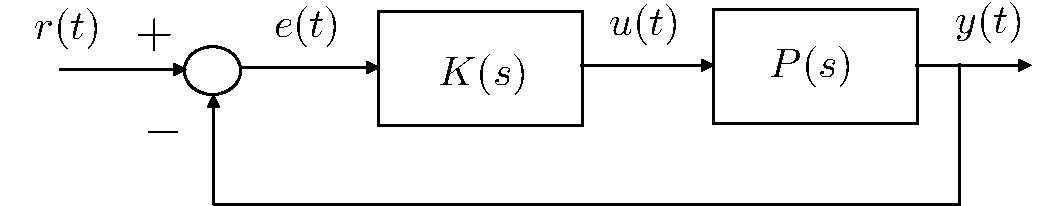
\includegraphics[width=0.9\textwidth]{figures/chap7_svd_feedback}
%	\end{center}	
%	The transfer matrix is derived by noting that
%	\begin{align*}
%		& E = R-Y = R-PU = R-PKE \\
%		\implies & E + PKE = R \\
%		\implies & (I + PK) E = R \\
%		\implies & 	E(s) = (I-PK)^{-1}R(s) \\
%	\end{align*}
%\end{frame}
%
%%----------------------------------
%\begin{frame}\frametitle{Application:  MIMO Feedback Control}
%	Taking the norm of $E(s)$ gives
%	\begin{align*}
%		\norm{E(s)} 
%			&= \norm{(I-PK)^{-1}R(s)} \\
%			&\leq \norm{(I-PK)^{-1}}\norm{R(s)} \\
%			&= \frac{1}{\underline{\sigma}(I-PK)}\norm{R(j\omega)},
%	\end{align*}
%	where $\underline{\sigma}(I-PK)(s)$ is the smallest singular value of $I-P(s)K(s)$.
%
%
%
%
%
%	\[ \norm{(I - PK)^{-1} } \]
%	\[ \norm{A^{-1} } = \frac{1}{\sigma(I-PK)} \]
%	\newpage
%	want
%	
%	\begin{align*}
%	\vec{\sigma}((I+PK)^{-1}) &\leq \gamma(j\omega)\\
%	= \frac{1}{\sigma(I+PK)} &\leq \gamma(j\omega)\\
%	\frac{1}{\gamma(j\omega)} &\leq \sigma(I+PK) \leq \sigma(I) + \vec{sigma}(PK)\\
%	&= 1 + \vec{\sigma}(PK)\\
%	\therefore \vec{\sigma}(PK) \leq \frac{1}{\gamma(j\omega)} - 1
%	\end{align*}
%	
%	
%	use the fact that
%	\[ \sigma(Q+R) \leq \sigma(Q) + \vec{\sigma}(R) \]
%	
%\end{frame}

%----------------------------------
\begin{frame}\frametitle{Application:  MIMO Communication}
	Consider the MIMO communication system modeled by
	\[ 
		\underbrace{
			Y(j\omega)
		}_{p\times 1} 
		= \underbrace{
			H(j\omega)
		  }_{1\times m}
		  \underbrace{
		  	X(j\omega)
		  }_{m\times 1} 
	\]
	
	\vfill
	
	What is the maximum gain of the system?
	\begin{align*}
		\norm{Y(j\omega)} 
			= \norm{H(j\omega)X(j\omega)} 
			\leq \norm{H(j\omega)}\norm{X(j\omega)} 
	\end{align*}
	Therefore, the maximum gain is given by
	\begin{align*}
		\gamma_{\max}(j\omega) 
			&=  \max_{X(j\omega) \neq 0}
					\frac{\norm{H(j\omega)X(j\omega)}}{\norm{X(j\omega)}} \\
		&= \norm{H(j\omega)}\\
		&= \bar{\sigma}(H(j\omega)),
	\end{align*}
	where $\bar{\sigma}(H(j\omega))$ is the maximum singular value of $H(j\omega)$.
\end{frame}

%----------------------------------
\begin{frame}\frametitle{Application:  MIMO Communication}
	How do you achieve this gain?
	Since 
	\[
		H(j\omega) 
			= \Sigma \sigma_k(j\omega)\ubf_k(j\omega)\vbf_k^H(j\omega),
	\]
	letting
	\[ 
		X(j\omega) = \vbf_1(j\omega) 
	\]
	maximizes the gain in the system over the set 
	$\norm{X(j\omega) } = 1$	.
\end{frame}




\end{document}